\chapter{Comparaci\'on de algoritmos}

\section{Tiempo de ejecuci\'on}
\subsection{Euclides Clasico}
\begin{table}[H]
\label{tablax}
\begin{center}
\begin{tabular}{|c|c|c|}
\hline 
a&b&time \\
\hline
938492342349723492374234723&6823234234232423234&0.000337\\\hline
548674568475645867&534653645634&0.0004\\\hline
2323423324&242342&7.1e-05\\\hline
23423&2342&0.000105\\\hline
234&123&3.7e-05\\\hline
\end{tabular}
\end{center}
\caption{Eficiencia de ejecuci\'on}
\end{table}
%-------------------------------------------------
%euclides con menor resto
\subsection{Euclides Menor Resto}
\begin{table}[H]
\label{tablax}
\begin{center}
\begin{tabular}{|c|c|c|}
\hline 
a&b&time \\
\hline
938492342349723492374234723&6823234234232423234&0.000382\\\hline
548674568475645867&534653645634&0.000232\\\hline
2323423324&242342&0.000133\\\hline
23423&2342&0.000106\\\hline
234&123&0.000121\\\hline
\end{tabular}
\end{center}
\caption{Eficiencia de ejecuci\'on}
\end{table}
%binario

\subsection{Binario Euclides}
\begin{table}[H]
\label{tablax}
\begin{center}
\begin{tabular}{|c|c|c|}
\hline 
a&b&time \\
\hline
938492342349723492374234723&6823234234232423234&0.000513\\\hline
548674568475645867&534653645634&0.000198\\\hline
2323423324&242342&0.000101\\\hline
23423&2342&6.9e-05\\\hline
234&123&5.2e-05\\\hline
\end{tabular}
\end{center}
\caption{Eficiencia de ejecuci\'on}
\end{table}


\subsection{Euclides extendido}
\begin{table}[!h]
\label{tablax}
\begin{center}
\begin{tabular}{|c|c|c|}
\hline 
a&b&time \\
\hline
938492342349723492374234723&6823234234232423234&0.000599\\\hline
548674568475645867&534653645634&0.000333\\\hline
2323423324&242342&0.000126\\\hline
23423&2342&8.2e-05\\\hline
234&123&0.000169\\\hline
\end{tabular}
\end{center}
\caption{Eficiencia de ejecuci\'on}
\end{table}


%\begin{figure}[H]
% \centering
% 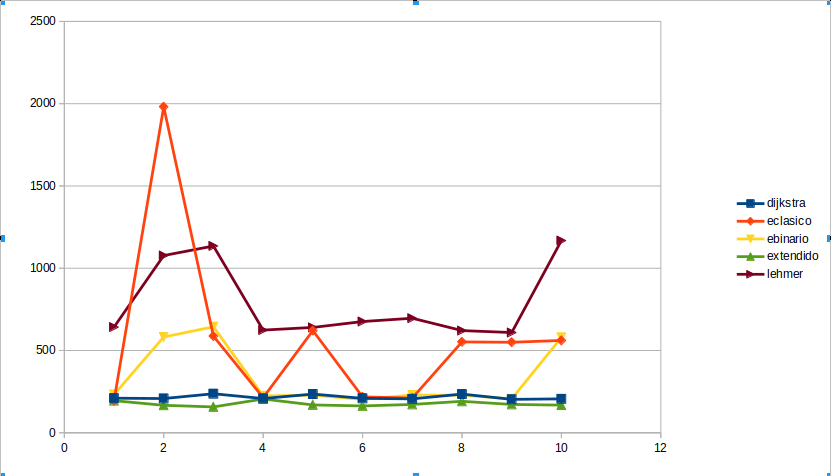
\includegraphics[scale=0.4]{pictures/32bits.png}
 % 32bits.png: 0x0 pixel, 300dpi, 0.00x0.00 cm, bb=
% \caption{Tiempo de ejecución de 32-Bits}
% \label{fig:1}
%\end{figure}



%\begin{figure}[h]
% \centering
% 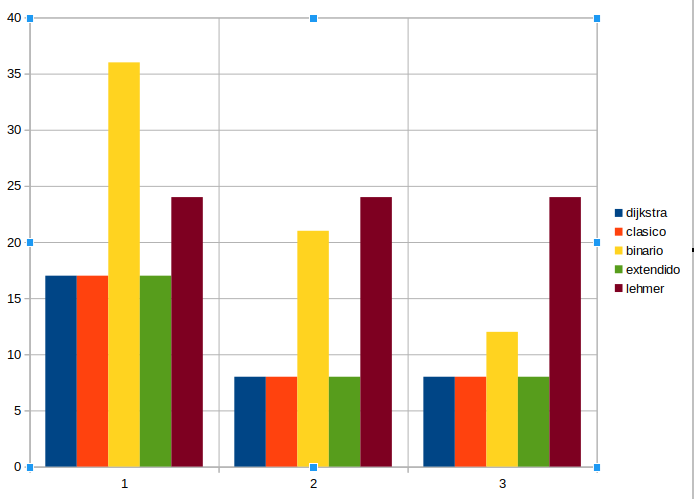
\includegraphics[scale=0.4]{pictures/iteracion.png}
 % iteracion.png: 0x0 pixel, 300dpi, 0.00x0.00 cm, bb=
% \caption{Nro de Iteraciones en 32, 16 y 8 bits}
% \label{fig:2}
%\end{figure}


\section{Comparacion de Tiempo de ejecucion}
\begin{table}[H]
\label{tablax}
\begin{center}
\begin{tabular}{|c|c|c|}
\hline 
i&a&b \\
\hline
1&938492342349723492374234723&6823234234232423234\\\hline
2&548674568475645867&534653645634\\\hline
3&2323423324&242342\\\hline
4&23423&2342\\\hline
5&234&123\\\hline
\end{tabular}
\end{center}
\caption{comparacion de tiempo}
\end{table}

\begin{figure}
    \centering
    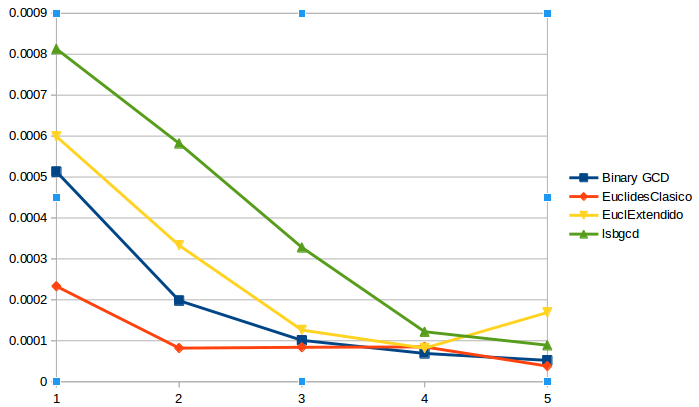
\includegraphics[scale=0.4]{pictures/dispersion.png}
    \caption{Caption conparacion de tiempo }
    
    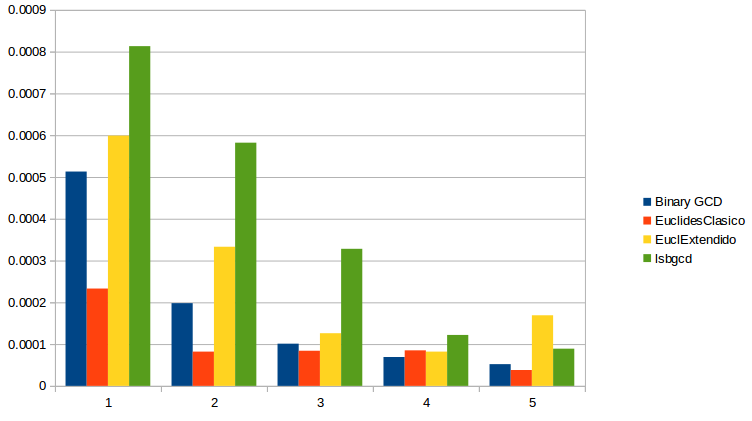
\includegraphics[scale=0.4]{pictures/barras.png}
    \caption{Caption comparacion de tiempo}
    
    \label{fig:my_label}
\end{figure}

%\begin{figure}[h]
% \centering
% 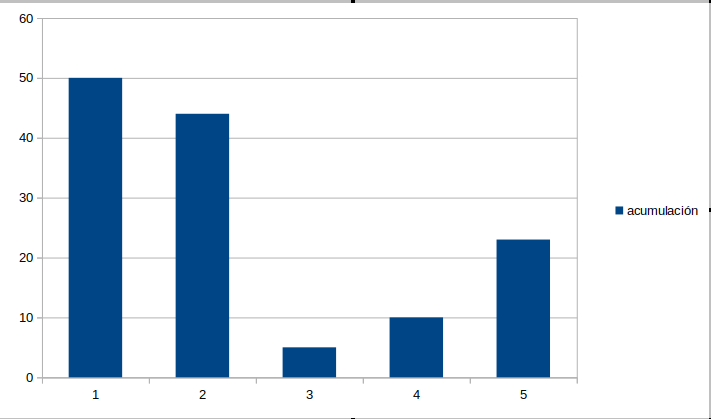
\includegraphics[scale=0.4]{pictures/acmulac.png}
 % acmulac.png: 0x0 pixel, 300dpi, 0.00x0.00 cm, bb=
% \caption{Acumulación de variable de todos los algoritmos}
% \label{fig:3}
%\end{figure}

